\chapter{Methodology and System Design}

This chapter details the design and architecture of the decentralized LoRa mesh system. It covers the hardware specifications, network topology, consensus mechanism, and the hybrid testbed approach used for validation.

\section{System Specifications}

The system is designed as a hybrid of physical hardware and software-simulated nodes.

\subsection{Physical Node Specifications}
Each physical node consists of:
\begin{itemize}
\item \textbf{Microcontroller}: ESP32 (Dual-core 240 MHz, 520 KB SRAM).
\item \textbf{Radio}: Semtech SX1276 LoRa transceiver.
\item \textbf{Sensors}:
    \begin{itemize}
    \item GPS for location tracking.
    \item MPU6050 IMU for motion and fall detection.
    \item MAX30102 for heart rate (HR) and blood oxygen saturation (SpO2).
    \end{itemize}
\item \textbf{Firmware}: C++ based implementation of the blockchain and consensus logic.
\end{itemize}

\subsection{Virtual Node Specifications}
Virtual nodes are software-simulated in Python to enable large-scale testing. They run the same logic as the physical nodes, including blockchain consensus and federated learning, but use a simulated LoRa channel model for communication.

\section{Network Topology and Scalability}

To ensure the system can scale to 50+ nodes, several strategies are employed.

\subsection{Partial Mesh Topology}
Instead of a full mesh where every node connects to every other node ($O(N^2)$ message complexity), each node in this system connects to only $\lfloor\sqrt{N}\rfloor$ nearest neighbors. This reduces the per-round message count from $O(N^2)$ to $O(N\sqrt{N})$.

\subsection{Gossip Propagation}
Blocks and weight updates are spread through the network using a gossip protocol with a fanout of 3. This ensures that a block reaches all $N$ nodes in $O(\log N)$ hops, providing robustness against node failures and network partitions.

\section{System Architecture}

The system architecture follows a decentralized model where physical and virtual nodes interact through a unified consensus and learning framework. Figure \ref{fig:methodology_tikz} illustrates the data flow and component interaction.

\begin{figure}[H]
\centering
\begin{tikzpicture}[
    node distance=1.5cm,
    base/.style={draw, minimum width=3cm, minimum height=1cm, align=center, rounded corners},
    physical/.style={base, fill=blue!10},
    process/.style={base, fill=green!10},
    virtual/.style={base, fill=orange!10},
    arrow/.style={-Stealth, thick}
]
    % Physical layer
    \node (sensors) [physical] {Physical Sensors\\(GPS, IMU, MAX30102)};
    \node (esp32) [physical, right=of sensors] {ESP32 Node\\(Blockchain + LoRa)};
    
    % Communication
    \node (lora) [process, below=of esp32] {LoRa Mesh / FHSS};
    \node (mqtt) [process, left=of lora] {MQTT Bridge};
    
    % Virtual layer
    \node (vnodes) [virtual, below=of mqtt] {Virtual Node Mesh\\(Python Simulation)};
    
    % Logic layers
    \node (poa) [process, right=of vnodes] {Weighted PoA\\Consensus};
    \node (fl) [process, below=of poa] {Federated Learning\\(Hierarchical FedAvg)};

    % Connections
    \draw [arrow] (sensors) -- (esp32);
    \draw [arrow] (esp32) -- (lora);
    \draw [arrow] (lora) -- (mqtt);
    \draw [arrow] (mqtt) -- (vnodes);
    \draw [arrow] (vnodes) -- (poa);
    \draw [arrow] (esp32) |- (poa);
    \draw [arrow] (poa) -- (fl);
    \draw [arrow] (fl) -| (vnodes);
\end{tikzpicture}
\caption{System Methodology and Component Interaction Flow}
\label{fig:methodology_tikz}
\end{figure}

\section{Consensus Mechanism: Weighted PoA}

The Proof-of-Authority (PoA) consensus mechanism uses a 5-check validator pipeline to ensure the integrity of proposed blocks.

\begin{algorithm}[H]
\caption{PoA Block Validator Pipeline}
\label{alg:poa_validator}
\begin{algorithmic}[1]
\REQUIRE Proposed Block $B$, Current Chain $C$
\STATE \textbf{Check 1:} Verify $B.signature$ using $Public\_Key(B.author)$ \COMMENT{ECDSA P-256}
\IF{Signature is Invalid} \RETURN REJECT \ENDIF
\STATE \textbf{Check 2:} Recompute $Hash(B.payload)$ and compare with $B.hash$ \COMMENT{SHA-256}
\IF{Hash Mismatch} \RETURN REJECT \ENDIF
\STATE \textbf{Check 3:} Verify $B.prev\_hash == C.tip\_hash$
\IF{Prev\_Hash Mismatch} \RETURN REJECT \ENDIF
\STATE \textbf{Check 4:} Verify $B.frame\_counter > C.last\_seen\_counter(B.author)$
\IF{Counter Not Greater} \RETURN REJECT \ENDIF
\STATE \textbf{Check 5:} Verify $B.anomaly\_score \leq 0.7$ \COMMENT{TinyML Model Gate}
\IF{Anomaly Score Too High} \RETURN REJECT \ENDIF
\STATE \RETURN APPROVE
\end{algorithmic}
\end{algorithm}

\subsection{Reputation-Weighted Voting}
Each node has a reputation score (0.0 to 1.0). A block is approved if the sum of the reputation weights of the nodes voting YES exceeds 51\% of the total weight in the validator set.

\section{Federated Learning Architecture}

The system uses a hierarchical federated averaging approach to reduce global communication overhead.

\subsection{Hierarchical FedAvg}
Nodes are clustered into $k = \lfloor\sqrt{N}\rfloor$ groups based on physical proximity. Intra-cluster averaging is performed first, and only the cluster-head weight vectors are shared for global aggregation. This reduces global communications from $O(N)$ to $O(\sqrt{N})$ per round.

\subsection{Differential Privacy Implementation}
Before broadcasting weight updates, nodes add Gaussian noise calibrated to a specific privacy budget ($\epsilon$). This ensures that an individual's raw physiological data cannot be reconstructed from the shared model updates.

\section{Hybrid Testbed Integration}

The physical and virtual nodes are integrated using an MQTT bridge. Physical ESP32 nodes publish blocks to an MQTT broker, which are then injected into the Python simulation. Conversely, blocks from the virtual mesh can be pushed back to the physical nodes, allowing for end-to-end validation of the consensus logic across a heterogeneous network.

\begin{figure}[H]
	\centering
	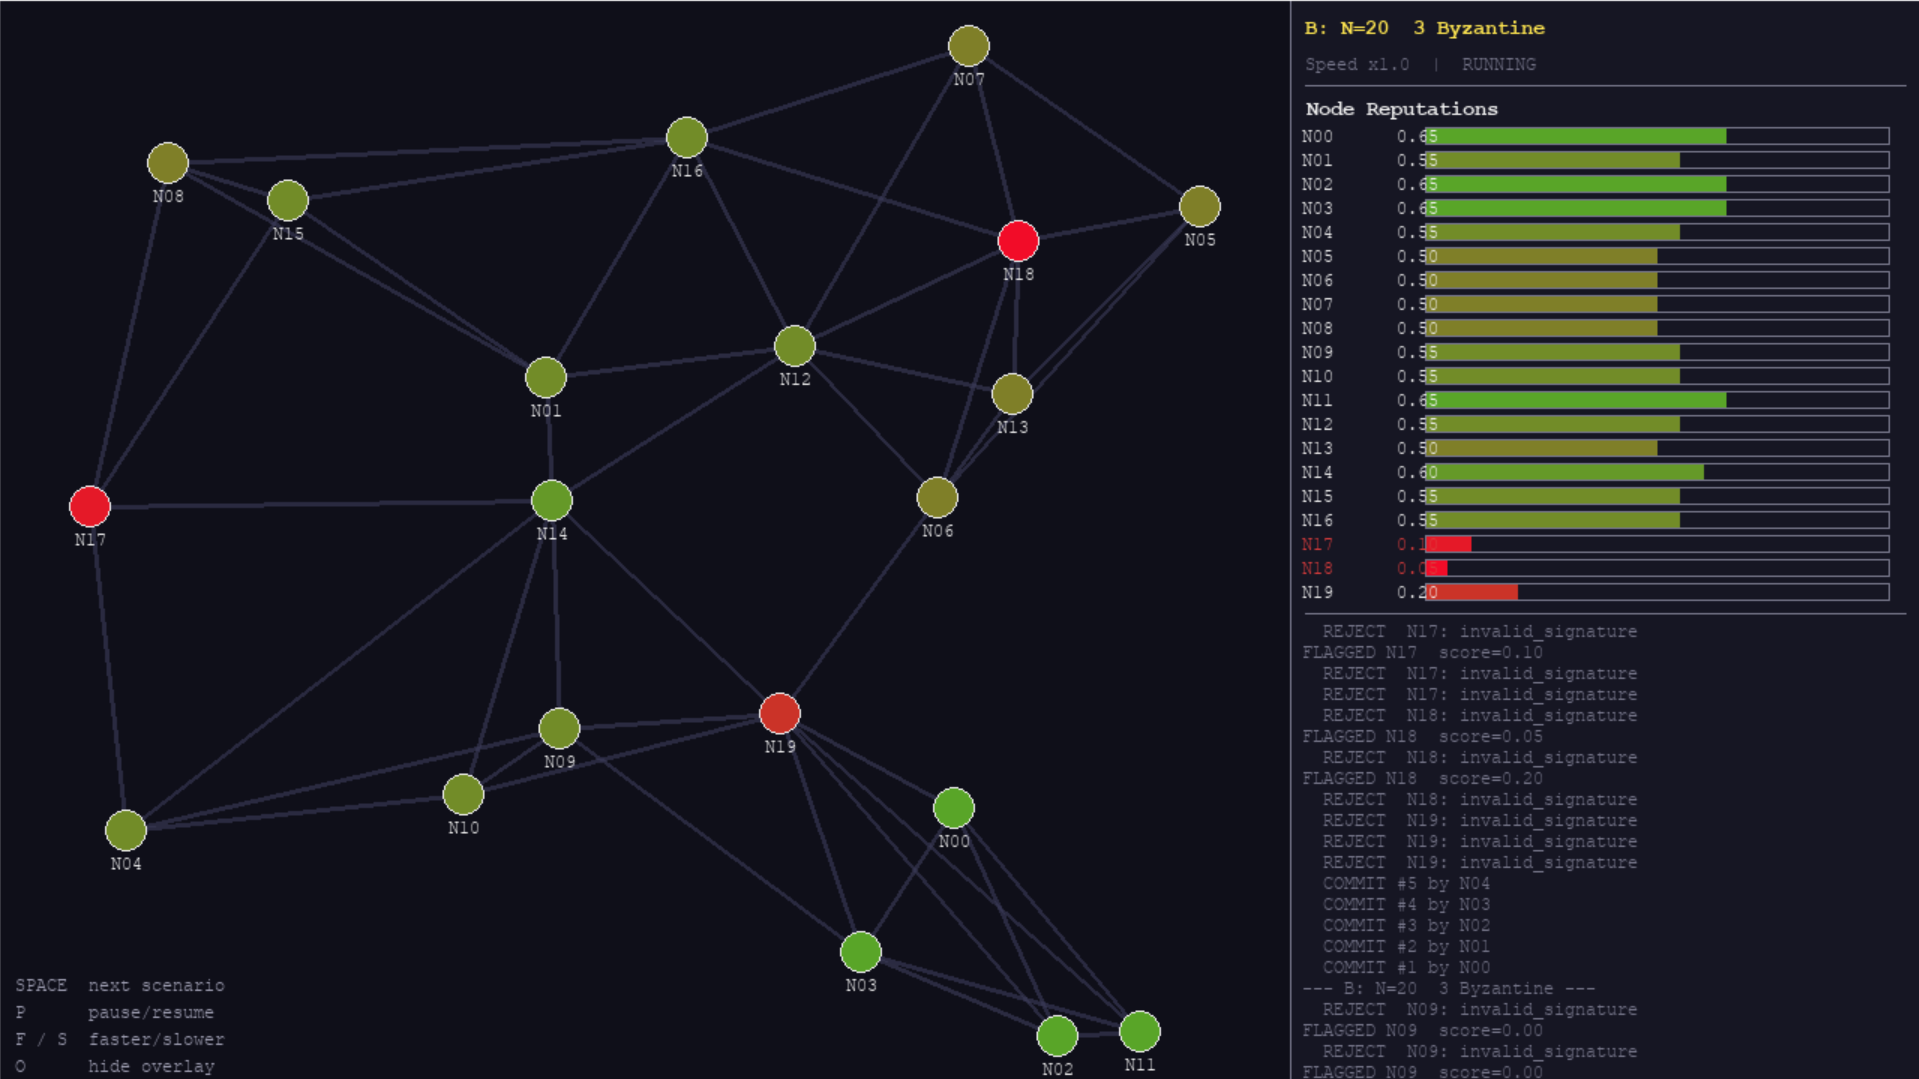
\includegraphics[width=0.8\textwidth]{Figures/hybrid_testbed.png}
	\caption{Hybrid Testbed Architecture: Physical and Virtual Node Integration}
	\label{fig:hybrid_testbed}
\end{figure}

\section{Summary}

This chapter described the design of the decentralized system, focusing on its scalability and security features. The use of a partial mesh, hierarchical FL, and a robust PoA consensus mechanism ensures that the system is suitable for large-scale, infrastructure-independent deployments. The next chapter will detail the implementation of these components.